% Memoria del proyecto postgres-production-lab
% Compilar desde la carpeta docs/ con:  latexmk -pdf memoria.tex   (o pdflatex dos veces)
\documentclass[11pt, a4paper, titlepage]{article}

% --- PAQUETES DE CONFIGURACIÓN ---
\usepackage[spanish, es-tabla]{babel}
\usepackage[utf8]{inputenc}
\usepackage[T1]{fontenc}
\usepackage{geometry}
\geometry{top=2.5cm, bottom=2.5cm, left=3cm, right=3cm}
\usepackage{graphicx}
\graphicspath{{./}}
\usepackage{booktabs}
\usepackage{array}
\usepackage{tabularx}
\usepackage{xcolor}
\usepackage{listings}
\usepackage{fancyhdr}
\usepackage{caption}
\usepackage{float} % permite [H] para fijar las tablas junto a su texto
% hyperref siempre el último; plainpages=false evita el aviso de "destination ... already used"
\usepackage[plainpages=false,pdfpagelabels]{hyperref}

% El BOM que añade Windows al principio de los scripts no se imprime
\DeclareUnicodeCharacter{FEFF}{}

% --- CABECERAS Y PIES DE PÁGINA ---
\pagestyle{fancy}
\setlength{\headheight}{14pt}
\fancyhf{}
\fancyhead[L]{\small Laboratorio de PostgreSQL en producción}
\fancyhead[R]{\small Proyecto personal}
\fancyfoot[C]{\thepage}

\hypersetup{
    colorlinks=true,
    linkcolor=black,
    citecolor=blue,
    urlcolor=blue,
    pdftitle={Laboratorio de PostgreSQL en producción},
    pdfauthor={Bogdan Turcu}
}

% --- LISTADOS DE CÓDIGO ---
\lstdefinelanguage{PowerShell}{
    morekeywords={foreach, in, if, else, function, param, return},
    sensitive=false,
    morecomment=[l]{\#},
    morecomment=[s]{<\#}{\#>},
    morestring=[b]",
    morestring=[b]'
}
\lstset{
    basicstyle=\ttfamily\small,
    keywordstyle=\color{blue!60!black},
    commentstyle=\color{green!40!black},
    stringstyle=\color{red!55!black},
    showstringspaces=false,
    frame=single,
    rulecolor=\color{black!30},
    xleftmargin=0.4cm,
    xrightmargin=0.2cm,
    aboveskip=0.3cm,
    belowskip=0.3cm,
    columns=fullflexible,
    keepspaces=true,
    breaklines=true,
    literate={á}{{\'a}}1 {é}{{\'e}}1 {í}{{\'i}}1 {ó}{{\'o}}1 {ú}{{\'u}}1 {ñ}{{\~n}}1
             {Á}{{\'A}}1 {É}{{\'E}}1 {Í}{{\'I}}1 {Ó}{{\'O}}1 {Ú}{{\'U}}1 {Ñ}{{\~N}}1
             {}{}0 % BOM de los scripts de Windows
}
\renewcommand{\lstlistingname}{Listado}

% Salida de un comando, sin colores
\lstdefinestyle{salida}{language={}, basicstyle=\ttfamily\footnotesize}

% Evita líneas que se salen del margen con nombres de comandos largos
\setlength{\emergencystretch}{3em}

% Nombre de un comando, fichero o variable
\newcommand{\cod}[1]{\texttt{#1}}

% --- INICIO DEL DOCUMENTO ---
\begin{document}

% ==========================================
% PORTADA
% ==========================================
\hypersetup{pageanchor=false} % la portada no necesita ancla de página
\begin{titlepage}
    \centering
    \vspace*{1cm}
    {\Huge\bfseries Proyecto Personal\par}
    \vspace{0.5cm}
    {\Large Administración de Bases de Datos en Producción\par}
    \vspace{0.3cm}
    {\large PostgreSQL \textperiodcentered{} Linux \textperiodcentered{} Automatización\par}

    \vspace{2.5cm}
    \rule{\linewidth}{0.5mm} \\[0.4cm]
    {\huge\bfseries Laboratorio de PostgreSQL en Producción\par}
    \vspace{0.2cm}
    {\Large Alta disponibilidad, replicación, copias de seguridad y operación de un clúster PostgreSQL 16\par}
    \rule{\linewidth}{0.5mm} \\[1.5cm]

    \begin{minipage}{0.48\textwidth}
        \begin{flushleft} \large
            \textbf{Repositorio:}\\
            \small\href{https://github.com/bogdanturcu13/postgres-production-lab}{github.com/bogdanturcu13/\\postgres-production-lab}\\[0.3cm]
            \large\textbf{Fecha:}\\
            Octubre de 2026
        \end{flushleft}
    \end{minipage}
    \hfill
    \begin{minipage}{0.48\textwidth}
        \begin{flushright} \large
            \textbf{Autor:}\\
            BOGDAN TURCU\\[0.3cm]
            \textbf{Estudios:}\\
            Grado en Ingeniería Informática
        \end{flushright}
    \end{minipage}
\end{titlepage}
\hypersetup{pageanchor=true}


% ==========================================
% TABLA DE CONTENIDOS
% ==========================================
\pagenumbering{roman}

\vspace{0.5cm}
\tableofcontents
\newpage
\pagenumbering{arabic}

% ==========================================
% SECCIÓN 1: INTRODUCCIÓN
% ==========================================
\section{Introducción y Objetivos}

Este proyecto es un laboratorio personal para aprender a administrar PostgreSQL como se hace en un entorno de producción. La idea no es solo instalar una base de datos, sino montar un entorno parecido al de una empresa, operarlo día a día y romperlo a propósito para aprender a diagnosticar y arreglar los problemas, igual que lo haría un administrador de bases de datos (DBA) o un ingeniero de fiabilidad (SRE).

PostgreSQL es un sistema gestor de bases de datos relacional de código abierto. Funciona con un modelo cliente-servidor: el servidor guarda los datos y atiende las consultas SQL que le envían las aplicaciones (los clientes) por la red. Un entorno de \textbf{producción} es aquel en el que la base de datos da servicio real a usuarios o aplicaciones, de modo que cualquier caída o pérdida de datos tiene consecuencias. El \textbf{DBA} (\textit{Database Administrator}) es quien se encarga de que ese servidor funcione, rinda y no pierda datos. El \textbf{SRE} (\textit{Site Reliability Engineering}) es un enfoque de operación nacido en Google que aplica técnicas de ingeniería de software, sobre todo la automatización y la medición, a mantener los servicios fiables.

Administrar una base de datos en producción va mucho más allá de escribir consultas SQL. Hay que garantizar que el servicio siga disponible cuando falla un servidor, que los datos se puedan recuperar después de un error humano, que el rendimiento se mantenga a medida que crecen los datos y que cualquier cambio se aplique sin interrumpir el servicio. Son competencias difíciles de adquirir sin un entorno en el que practicar y, sobre todo, en el que equivocarse sin consecuencias.

Los objetivos del proyecto son los siguientes:

\begin{itemize}
    \item \textbf{Administración:} Instalar, configurar y mantener PostgreSQL en producción.
    \item \textbf{Alta disponibilidad:} Montar un clúster con Patroni y etcd, y comprobar su comportamiento ante fallos reales.
    \item \textbf{Replicación:} Configurar replicación física (\textit{streaming}) y lógica, y conocer sus limitaciones.
    \item \textbf{Copias de seguridad:} Hacer backups, restauraciones y recuperación ante desastres con pgBackRest, incluida la recuperación a un instante concreto (PITR) y la medición del RTO y el RPO.
    \item \textbf{Monitorización y rendimiento:} Monitorizar el clúster, analizar consultas lentas y planificar la capacidad.
    \item \textbf{Mantenimiento:} \cod{VACUUM}, \cod{ANALYZE}, \cod{REINDEX}, control del \textit{bloat} y ajuste de autovacuum.
    \item \textbf{Cambios en producción:} Aplicar parches y actualizar de versión (de la 16 a la 18) siguiendo un proceso formal de gestión de cambios.
    \item \textbf{Incidencias:} Resolver incidencias, analizar su causa raíz y documentarlas como postmortems siguiendo ITIL.
    \item \textbf{Automatización:} Automatizar todo con Bash y Ansible, hasta poder destruir el laboratorio y reconstruirlo desde cero.
\end{itemize}

El resultado final es un repositorio público en GitHub\footnote{\url{https://github.com/bogdanturcu13/postgres-production-lab}} con la infraestructura como código, los procedimientos de operación (\textit{runbooks}), los informes de incidencias (postmortems) y la documentación del proyecto.

\subsection{Conceptos Básicos}

Antes de entrar en el laboratorio conviene aclarar los conceptos que aparecen en los objetivos. Los más específicos de cada fase se explican en su apartado correspondiente.

\paragraph{Alta disponibilidad.} Es la capacidad de un sistema de seguir dando servicio aunque falle alguno de sus componentes. En una base de datos se consigue con varias copias del servidor: un \textbf{primario}, que es el único que acepta escrituras, y una o varias \textbf{réplicas}, que mantienen una copia actualizada de los datos. Si el primario cae, una réplica se promociona a primario; a esto se le llama \textbf{failover} cuando ocurre por un fallo y \textbf{switchover} cuando se hace de forma planificada, por ejemplo para hacer un mantenimiento. Al conjunto de servidores que trabajan juntos se le llama \textbf{clúster}, y a cada uno de ellos, \textbf{nodo}.

\paragraph{WAL y replicación.} PostgreSQL no escribe los cambios directamente en los ficheros de datos. Primero los anota en un registro secuencial llamado \textbf{WAL} (\textit{Write-Ahead Log}) y solo después los aplica a los datos. Gracias a eso, si el servidor se apaga de golpe, al arrancar repasa el WAL y recupera los cambios que no le dio tiempo a aplicar. El WAL es también la base de casi todo lo demás: la \textbf{replicación física} consiste en enviar el WAL del primario a las réplicas para que apliquen exactamente los mismos cambios, y la \textbf{replicación lógica} envía en su lugar los cambios fila a fila, lo que permite copiar solo algunas tablas o hacia otra versión de PostgreSQL.

\paragraph{Copias de seguridad y recuperación.} La alta disponibilidad no sustituye a las copias de seguridad: si alguien borra una tabla por error, el borrado se replica a todas las réplicas en milisegundos. Las copias de seguridad sirven para volver atrás. Si además se guarda todo el WAL generado desde la copia, se puede restaurar la base de datos a cualquier instante concreto, por ejemplo justo antes del borrado; es lo que se conoce como \textbf{PITR} (\textit{Point-In-Time Recovery}). La recuperación ante desastres (DR) se mide con dos valores:
\begin{itemize}
    \item \textbf{RTO} (\textit{Recovery Time Objective}): cuánto tiempo se tarda en volver a dar servicio.
    \item \textbf{RPO} (\textit{Recovery Point Objective}): cuántos datos se pierden, medido en tiempo (por ejemplo, los últimos 5 minutos).
\end{itemize}

\paragraph{Mantenimiento.} En PostgreSQL, cuando una fila se modifica o se borra, la versión antigua no desaparece en el momento, sino que se queda ocupando espacio hasta que se limpia. \cod{VACUUM} hace esa limpieza, \cod{ANALYZE} actualiza las estadísticas que usa PostgreSQL para decidir cómo ejecutar cada consulta y \cod{REINDEX} reconstruye los índices. El \textit{bloat} es el espacio desperdiciado cuando esa limpieza no se hace a tiempo, y autovacuum es el proceso que la hace automáticamente.

\paragraph{Operación.} Un \textbf{runbook} es un procedimiento paso a paso para una tarea concreta (por ejemplo, reconstruir una réplica), escrito para que cualquiera pueda seguirlo en mitad de una incidencia. Un \textbf{postmortem} es el informe que se escribe después de una incidencia para explicar qué pasó, por qué y qué se va a cambiar para que no se repita. \textbf{ITIL} es un conjunto de buenas prácticas de gestión de servicios de TI muy extendido en empresas, que distingue entre \textit{incidentes} (algo ha fallado y hay que restablecer el servicio), \textit{problemas} (la causa de fondo de uno o varios incidentes) y \textit{cambios} (cualquier modificación planificada en producción). Por último, la \textbf{infraestructura como código} consiste en describir los servidores y su configuración en ficheros de texto versionados, de forma que se puedan reconstruir de manera automática y repetible; en este proyecto se hace con scripts y con Ansible, una herramienta que configura servidores remotos a través de SSH.

% ==========================================
% SECCIÓN 2: ARQUITECTURA
% ==========================================
\section{Arquitectura del Laboratorio}

El laboratorio se ejecuta en un único portátil con Windows 11 Pro, sobre el hipervisor Hyper-V. Está formado por cuatro máquinas virtuales con Rocky Linux 9:

\begin{itemize}
    \item \textbf{\cod{pg1}, \cod{pg2} y \cod{pg3}:} Los tres nodos de base de datos. Uno hará de primario y los otros dos de réplicas.
    \item \textbf{\cod{infra}:} La máquina de infraestructura, que concentra los servicios de apoyo.
\end{itemize}

La tabla \ref{tab:componentes} resume para qué sirve cada componente. Cada uno se instala y se explica en detalle en la fase en la que se usa.

\begin{table}[H]
\centering
\small
\begin{tabular}{llp{9.2cm}}
\toprule
\textbf{Componente} & \textbf{Máquina} & \textbf{Función} \\
\midrule
PostgreSQL 16 & \cod{pg1}--\cod{pg3} & El servidor de base de datos. \\
Patroni & \cod{pg1}--\cod{pg3} & Vigila PostgreSQL en cada nodo y, si cae el primario, promociona una réplica de forma automática. \\
etcd & \cod{pg1}--\cod{pg3} & Almacén de datos distribuido que usa Patroni para ponerse de acuerdo sobre qué nodo es el primario. Funciona por \textbf{quorum}: solo toma decisiones si responde la mayoría de sus nodos (2 de 3), lo que evita que dos nodos se crean primarios a la vez. \\
HAProxy & \cod{infra} & Balanceador de carga: recibe las conexiones de los clientes y las envía al nodo que sea primario en cada momento. \\
PgBouncer & \cod{infra} & \textit{Pooler} de conexiones: mantiene abiertas unas pocas conexiones con PostgreSQL y las reparte entre muchos clientes, porque cada conexión directa a PostgreSQL consume bastante memoria. \\
pgBackRest & \cod{infra} & Herramienta de copias de seguridad de PostgreSQL, con copias completas, diferenciales e incrementales y archivado del WAL. \\
MinIO & \cod{infra} & Almacenamiento de objetos compatible con Amazon S3, donde pgBackRest guarda las copias. \\
Prometheus & \cod{infra} & Recoge y guarda métricas (uso de CPU, conexiones, retraso de la replicación...) de todas las máquinas. \\
Alertmanager & \cod{infra} & Envía avisos cuando una métrica supera un umbral. \\
Grafana & \cod{infra} & Muestra las métricas en paneles gráficos. \\
Ansible & \cod{infra} & Automatiza la instalación y la configuración del resto de máquinas. \\
\bottomrule
\end{tabular}
\caption{Componentes del laboratorio.}
\label{tab:componentes}
\end{table}

Las cuatro máquinas comparten una red interna aislada, 10.10.10.0/24, en la que el propio Windows hace de puerta de enlace y traduce las direcciones (NAT) hacia la red real. Estos conceptos de red se explican en la sección \ref{sec:red}. La figura \ref{fig:arquitectura} resume la arquitectura.

\begin{figure}[H]
\centering
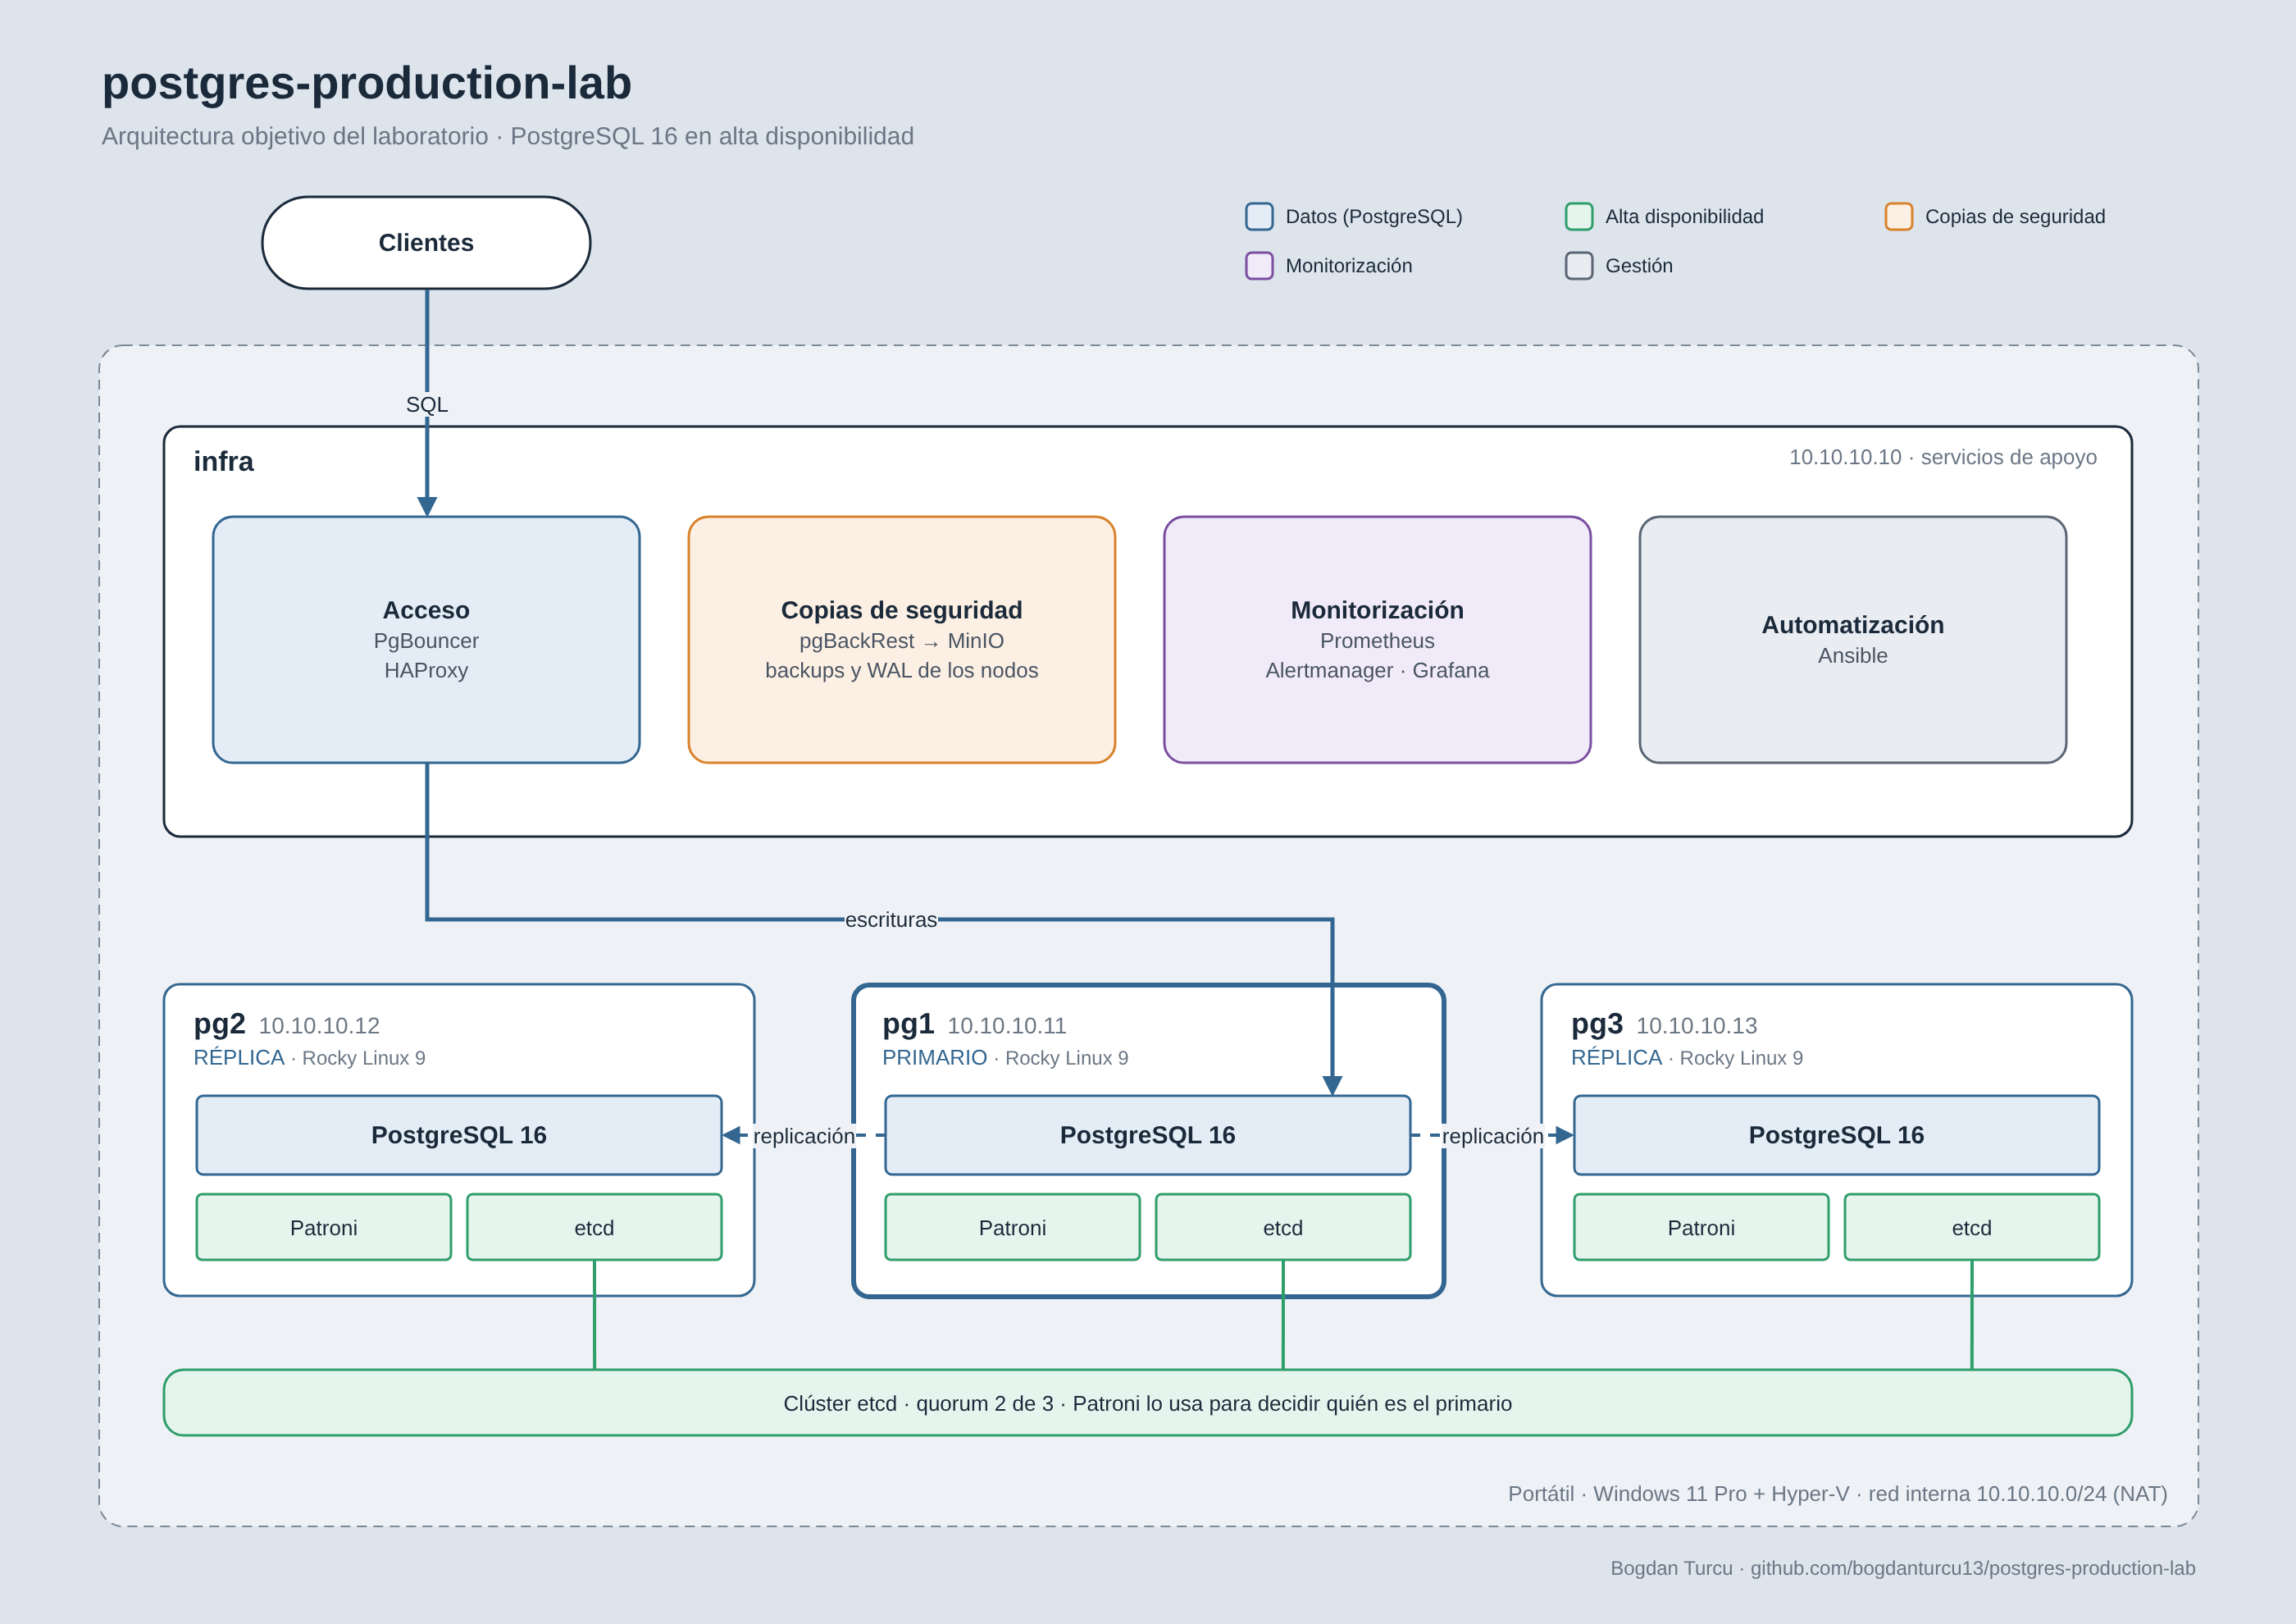
\includegraphics[width=\textwidth]{arquitectura.png}
\caption{Arquitectura del laboratorio.}
\label{fig:arquitectura}
\end{figure}

\subsection{Máquinas Virtuales}

Una \textbf{máquina virtual} (VM) es un ordenador simulado por software: tiene su propia CPU, memoria, discos y tarjeta de red virtuales, y en ella se instala un sistema operativo completo como si fuera un equipo físico. Varias máquinas virtuales pueden funcionar a la vez en un mismo equipo real, repartiéndose sus recursos. A cada procesador que se asigna a una máquina virtual se le llama \textbf{vCPU} (CPU virtual).

Todas las máquinas tienen un disco para el sistema operativo y otro distinto para los datos. Los motivos de esta separación se explican en la sección \ref{sec:vms}.

\begin{table}[H]
\centering
\small
\begin{tabular}{llccccl}
\toprule
\textbf{VM} & \textbf{IP} & \textbf{vCPU} & \textbf{RAM} & \textbf{Disco SO} & \textbf{Disco datos} & \textbf{Rol} \\
\midrule
\cod{infra} & 10.10.10.10 & 2 & 4 GB & 20 GB & 40 GB & Infraestructura \\
\cod{pg1}   & 10.10.10.11 & 2 & 3 GB & 20 GB & 20 GB & Base de datos \\
\cod{pg2}   & 10.10.10.12 & 2 & 3 GB & 20 GB & 20 GB & Base de datos \\
\cod{pg3}   & 10.10.10.13 & 2 & 3 GB & 20 GB & 20 GB & Base de datos \\
\bottomrule
\end{tabular}
\caption{Inventario de máquinas virtuales.}
\label{tab:inventario}
\end{table}

\subsection{Planificación por Fases}

El trabajo se divide en diez fases. Cada una tiene sus objetivos, un ejercicio en el que se provoca un fallo a propósito y un entregable en el repositorio. No se pasa a la siguiente fase hasta cumplir el criterio de salida de la anterior. Los términos propios de cada fase que aparecen en la tabla se explican al llegar a ella.

\begin{table}[H]
\centering
\small
\begin{tabular}{clp{8.2cm}}
\toprule
\textbf{Fase} & \textbf{Tema} & \textbf{Contenido} \\
\midrule
0 & Preparación & Máquinas virtuales, red, acceso SSH por clave y repositorio. \\
1 & Instalación & PostgreSQL 16 desde PGDG, memoria, logging, checkpoints, roles y PgBouncer. \\
2 & Replicación & Streaming replication, slots, modo síncrono y asíncrono, replicación lógica. \\
3 & Alta disponibilidad & Patroni, etcd y HAProxy. Switchover, failover y pérdida de quorum. \\
4 & Backups y DR & pgBackRest con MinIO, PITR, restauración completa, RTO y RPO. \\
5 & Monitorización & Prometheus, Grafana, alertas, análisis de consultas y capacidad. \\
6 & Mantenimiento & MVCC, \textit{bloat}, autovacuum, \cod{REINDEX} y \textit{wraparound}. \\
7 & Cambios & Parches con reinicio escalonado y actualización de la versión 16 a la 18. \\
8 & Incidencias e ITIL & Incidentes, problemas y cambios en ServiceNow, guardias y postmortems. \\
9 & Automatización & Roles de Ansible y reconstrucción completa del laboratorio. \\
\bottomrule
\end{tabular}
\caption{Fases del proyecto.}
\label{tab:fases}
\end{table}

\subsection{Estructura del Repositorio}

Todo lo que se hace en el laboratorio queda documentado o automatizado en el repositorio:

\begin{table}[H]
\centering
\small
\begin{tabular}{lp{10cm}}
\toprule
\textbf{Ruta} & \textbf{Contenido} \\
\midrule
\cod{docs/apuntes.md} & Cuaderno de trabajo con lo hecho en cada bloque, los problemas encontrados y su solución. Es la base de este documento. \\
\cod{docs/decisiones/} & Registro de decisiones de arquitectura (ADR, \textit{Architecture Decision Record}): documentos breves que explican por qué se ha elegido cada cosa frente a sus alternativas. \\
\cod{docs/preguntas.md} & Preguntas de repaso tipo entrevista técnica de cada fase. \\
\cod{docs/plantillas/} & Plantillas de runbook, postmortem y ADR. \\
\cod{scripts/} & Scripts para crear y preparar el laboratorio. \\
\cod{ansible/} & Automatización del despliegue (a partir de la Fase 1). \\
\cod{runbooks/}, \cod{postmortems/} & Procedimientos de operación e informes de incidencias. \\
\bottomrule
\end{tabular}
\caption{Estructura del repositorio.}
\label{tab:repositorio}
\end{table}

Cada tarea sigue el mismo método: primero se explica el concepto, después se ejecutan los pasos y por último se comprueba que funciona con comandos de verificación. Cuando algo falla, se diagnostica antes de aplicar una solución.

% ==========================================
% SECCIÓN 3: FASE 0
% ==========================================
\section{Fase 0: Preparación del Entorno}

En esta primera fase se prepara la base sobre la que se construye el resto del proyecto: el hipervisor, la red, las cuatro máquinas virtuales con su sistema operativo, el acceso remoto seguro y el repositorio. El criterio de salida es tener acceso SSH por clave entre todas las máquinas y el repositorio creado con su estructura.

\subsection{Equipo y Decisiones Previas}

El laboratorio se ejecuta en el siguiente equipo:

\begin{table}[H]
\centering
\small
\begin{tabular}{lp{9cm}}
\toprule
\textbf{Componente} & \textbf{Detalle} \\
\midrule
Procesador & Intel Core i5-11400H, 6 núcleos y 12 hilos \\
Memoria & 32 GB \\
Sistema operativo & Windows 11 Pro \\
Disco del laboratorio & Unidad E:, NVMe Crucial P2 (CT1000P2SSD8), con 484 GB libres \\
\bottomrule
\end{tabular}
\caption{Características del equipo.}
\label{tab:equipo}
\end{table}

El procesador tiene 6 núcleos físicos, pero cada uno puede ejecutar dos hilos a la vez gracias a una técnica llamada SMT (\textit{Simultaneous Multithreading}, o \textit{Hyper-Threading} en Intel), por eso el sistema ve 12. Con estos recursos cabe la arquitectura completa sin recortes: las cuatro máquinas suman 8 vCPU y 13 GB de RAM, y a Windows le quedan casi 19 GB.

\subsubsection{Hipervisor}

Para crear máquinas virtuales hace falta un \textbf{hipervisor}, que es el software que reparte el hardware real entre ellas y las mantiene aisladas unas de otras. Hay dos tipos:

\begin{itemize}
    \item \textbf{Tipo 1 (\textit{bare metal}):} Se ejecuta directamente sobre el hardware, sin un sistema operativo por debajo. Es el que se usa en los centros de datos. Ejemplos: Hyper-V, VMware ESXi, KVM.
    \item \textbf{Tipo 2:} Es una aplicación más que se ejecuta dentro de un sistema operativo. Es más sencillo de usar, pero añade una capa intermedia. Ejemplos: VirtualBox, VMware Workstation.
\end{itemize}

Se ha elegido \textbf{Hyper-V}, el hipervisor de Microsoft, que viene incluido en Windows 11 Pro. Aunque se activa desde Windows, es de tipo 1: al activarlo, lo primero que se carga al arrancar el equipo es el hipervisor, y Windows se ejecuta encima de él en la \textit{partición raíz}, una máquina virtual con privilegios especiales que gestiona los controladores y crea el resto de máquinas. Por eso parece que Windows sigue siendo el sistema principal, aunque en realidad no lo es.

Además, Hyper-V no choca con WSL2 (el subsistema de Windows para ejecutar Linux) ni con las funciones de seguridad de Windows 11 que se basan en la virtualización, como la integridad de memoria, que de hecho ya usan el hipervisor por debajo. VirtualBox, en cambio, tendría que funcionar encima de esa capa de Hyper-V y perdería bastante rendimiento de disco. Por último, Hyper-V se puede manejar entero con \textbf{PowerShell}, la consola y lenguaje de scripts de Windows, lo que permite automatizar la creación del laboratorio. Sus comandos se llaman \textit{cmdlets} y siguen el formato \textit{Verbo-Sustantivo}, como \cod{New-VM} (crear una máquina) o \cod{Get-VM} (consultarlas).

\subsubsection{Sistema Operativo}

Las máquinas usan \textbf{Rocky Linux 9}. Rocky es una copia gratuita y compatible 1:1 con Red Hat Enterprise Linux (RHEL), la distribución de Linux más habitual en grandes empresas y en banca: se compila a partir del mismo código fuente, así que los paquetes, las rutas y el comportamiento son los mismos. La diferencia con RHEL es que no requiere pagar una suscripción. Se eligió frente a Debian o Ubuntu porque obliga a trabajar con dos piezas de seguridad que están activadas por defecto en ese tipo de entornos: \textbf{SELinux}, que se explica en la sección \ref{sec:selinux}, y \textbf{firewalld}, el cortafuegos de la familia Red Hat, que organiza las reglas por servicios (por ejemplo, \cod{ssh}) en lugar de por puertos sueltos.

Las dos decisiones se documentan como ADR en el repositorio (apéndice \ref{ap:decisiones}).

\subsubsection{Disco}

Hay un detalle del disco que conviene tener presente. La unidad E: es un SSD NVMe (un SSD conectado directamente al bus PCI Express, mucho más rápido que los antiguos SATA) sin memoria DRAM propia. Los SSD de este tipo escriben primero en una pequeña zona rápida que hace de caché y, cuando se llena en escrituras largas y sostenidas, la velocidad cae bastante. Como las cuatro máquinas escriben en el mismo disco físico, habrá que tenerlo en cuenta al interpretar las métricas de disco en la Fase 5.

\subsection{Repositorio y Control de Versiones}

El proyecto se guarda en un repositorio de \textbf{Git}, un sistema de control de versiones que registra cada cambio en los ficheros como un \textit{commit}, con su autor, su fecha y un mensaje que lo describe. El repositorio se sube (\cod{git push}) a GitHub, donde es público desde el primer día. Por eso se crea con dos ficheros de configuración:

\begin{itemize}
    \item \textbf{\cod{.gitignore}:} Lista los ficheros que Git nunca debe subir: los discos virtuales, las ISO, las claves privadas y cualquier fichero de secretos.
    \item \textbf{\cod{.gitattributes}:} Fuerza los finales de línea de tipo LF. Windows termina cada línea de un fichero de texto con dos caracteres invisibles, CR y LF (\textit{CRLF}), mientras que Linux solo usa LF. Si un script editado en Windows llega a Linux con CRLF, el carácter CR sobrante hace que falle. La excepción son los scripts de PowerShell, que se dejan en CRLF porque se ejecutan en Windows.
\end{itemize}

\subsubsection{Problema: Error 403 al Subir Cambios}

En Git hay que distinguir dos cosas que no tienen nada que ver: la \textbf{identidad} con la que se firman los commits (un nombre y un correo, configurados con \cod{user.name} y \cod{user.email}) y la \textbf{cuenta} con la que uno se autentica en GitHub al subir los cambios. El problema vino de la segunda.

\begin{itemize}
    \item \textbf{Síntoma:} \cod{git push} devolvía \textit{Permission denied to ualbt635}. Git se autenticaba con la cuenta de GitHub de la universidad en lugar de con la personal.
    \item \textbf{Causa:} Al conectarse por HTTPS, Git usa las credenciales guardadas en el Administrador de credenciales de Windows. Ahí estaban las de la otra cuenta, y Git las reutilizaba sin preguntar.
    \item \textbf{Solución:} Se cambió HTTPS por SSH, con una clave y un alias por cuenta (\cod{github-personal} y \cod{github-uni}) en \cod{\textasciitilde/.ssh/config}. Así, la cuenta queda escrita en la propia dirección del repositorio, por ejemplo \cod{git@github-personal:\allowbreak bogdanturcu13/...}. La identidad de los commits se elige según la carpeta en la que está el repositorio con la directiva \cod{includeIf} de la configuración de Git, y la opción \cod{user.useConfigOnly} impide hacer un commit si no hay ninguna identidad configurada, en lugar de inventarse una.
\end{itemize}

\subsection{Configuración de Hyper-V}

Por defecto, Hyper-V guarda las máquinas y sus discos en la unidad C:, que solo tenía 14,5 GB libres. Antes de crear nada se movieron las rutas a la unidad E: desde PowerShell como administrador:

\begin{lstlisting}[language=PowerShell]
Enable-WindowsOptionalFeature -Online -FeatureName Microsoft-Hyper-V -All

New-Item -ItemType Directory -Path E:\HyperV\VHD, E:\HyperV\VMs, E:\HyperV\ISO -Force
Set-VMHost -VirtualHardDiskPath 'E:\HyperV\VHD' -VirtualMachinePath 'E:\HyperV\VMs'
Get-VMHost | Select-Object VirtualHardDiskPath, VirtualMachinePath
\end{lstlisting}

El primer comando activa Hyper-V; \cod{New-Item} crea las carpetas y \cod{Set-VMHost} cambia las rutas por defecto de los discos virtuales (ficheros \cod{.vhdx}) y de la configuración de las máquinas. En este equipo Hyper-V ya estaba activado: el primer comando devolvió \cod{RestartNeeded : False} y la propiedad \cod{HypervisorPresent} de \cod{Win32\_ComputerSystem} valía \cod{True}, así que no hizo falta reiniciar.

Por último, se descargó la imagen de instalación \cod{Rocky-9.8-\allowbreak x86\_64-\allowbreak minimal.iso}. Una imagen ISO es un fichero que contiene el contenido completo de un disco óptico, en este caso el instalador del sistema. La versión \textit{minimal} incluye solo lo imprescindible para instalar un servidor sin entorno gráfico.

\subsection{Red Interna con NAT}
\label{sec:red}

Antes de ver cómo se ha montado la red, conviene repasar los conceptos que intervienen:

\begin{itemize}
    \item \textbf{Dirección IP y máscara:} Cada equipo de la red tiene una dirección IP, como 10.10.10.11. La notación \cod{10.10.10.0/24} indica una red cuyos primeros 24 bits (los tres primeros números) son fijos, de modo que admite equipos desde 10.10.10.1 hasta 10.10.10.254. Es lo mismo que la máscara 255.255.255.0.
    \item \textbf{Puerta de enlace:} Es el equipo al que una máquina envía todo el tráfico dirigido a otras redes, por ejemplo a Internet. Hace de router.
    \item \textbf{NAT} (\textit{Network Address Translation}): Las direcciones 10.x.x.x son privadas y no se pueden usar en Internet. Con NAT, el router sustituye la dirección privada de origen de cada paquete por su propia dirección real y, cuando llega la respuesta, deshace el cambio para entregarla a la máquina correcta. Es lo mismo que hace el router de casa.
    \item \textbf{DHCP:} Protocolo que asigna direcciones IP automáticamente a los equipos que se conectan a una red.
    \item \textbf{DNS:} Sistema que traduce nombres como \cod{google.com} a direcciones IP. En el laboratorio se usan los servidores DNS públicos 1.1.1.1 (Cloudflare) y 8.8.8.8 (Google).
    \item \textbf{Switch virtual:} Igual que un switch físico conecta los equipos de una red local, un switch virtual conecta entre sí las tarjetas de red de las máquinas virtuales.
\end{itemize}

Las máquinas se conectan a un switch virtual \textbf{interno}, \cod{LabSwitch}. Al crearlo, Windows recibe una tarjeta de red virtual conectada a él, \cod{vEthernet (LabSwitch)}, en la que se le asigna la dirección 10.10.10.1. Windows hace así de puerta de enlace y de router con NAT hacia la red real. Con este diseño:

\begin{itemize}
    \item \textbf{Direcciones fijas:} Las IP de las máquinas no dependen de la red a la que esté conectado el portátil.
    \item \textbf{Aislamiento:} Las máquinas salen a Internet para instalar paquetes, pero nadie de fuera puede entrar en ellas.
    \item \textbf{Sin DHCP:} Cada máquina tiene su dirección configurada a mano, como en producción, donde los servidores tienen direcciones fijas para que los clientes sepan siempre dónde encontrarlos.
\end{itemize}

La alternativa sería un switch \textbf{externo}, que conecta las máquinas directamente a la red real como si fueran equipos enchufados al router. En ese caso recibirían la dirección del router de casa por DHCP, cambiarían al cambiar de red y quedarían expuestas al resto de dispositivos.

La red se crea con el script \cod{01-red.ps1} (apéndice \ref{ap:scripts}), que tiene solo tres comandos:

\begin{table}[H]
\centering
\small
\begin{tabular}{lp{10cm}}
\toprule
\textbf{Comando} & \textbf{Función} \\
\midrule
\cod{New-VMSwitch} & Crea el switch interno \cod{LabSwitch}. \\
\cod{New-NetIPAddress} & Asigna a Windows la IP 10.10.10.1/24 en ese switch. \\
\cod{New-NetNat} & Crea el NAT \cod{LabNAT} para la red 10.10.10.0/24. \\
\bottomrule
\end{tabular}
\caption{Comandos del script de red.}
\label{tab:red}
\end{table}

Para comprobar que funciona se usa \cod{Get-NetNat}, que muestra el NAT activo, y \cod{Test-Connection 10.10.10.1}, que hace \textit{ping} a la nueva dirección (envía un pequeño paquete y espera respuesta, para comprobar que un equipo es alcanzable). En PowerShell 5.1, la columna \cod{IPV4Address} de \cod{Test-Connection} muestra la IP de \textbf{origen} (la de la red real), no la de destino. Lo importante es que hay respuesta.

\begin{lstlisting}[style=salida]
Name                             : LabNAT
InternalIPInterfaceAddressPrefix : 10.10.10.0/24
Active                           : True
\end{lstlisting}

\subsubsection{Problemas Encontrados}

\begin{itemize}
    \item \textbf{Fallo al crear el switch:} \cod{New-VMSwitch} falló con el código \cod{0x800700B7} (\textit{No se puede crear un archivo que ya existe}) sin que existiera ningún switch ni adaptador con ese nombre. Como consecuencia también falló \cod{New-NetIPAddress}, porque no existía la tarjeta \cod{vEthernet (LabSwitch)}; el NAT sí se creó. Al repetir el comando, el switch se creó bien: fue un error puntual al registrar el adaptador virtual. Los posibles factores son restos de un adaptador de Hyper-V antiguo y controladores de VPN (Fortinet, Hamachi) en estado de error, que instalan filtros sobre todas las tarjetas de red del equipo.

    \item \textbf{Switch duplicado:} Al reintentar se crearon dos switches llamados \cod{LabSwitch}. Hyper-V lo permite porque identifica cada switch internamente por un Id único y no por su nombre. Se solucionó borrando ambos con \cod{Remove-VMSwitch -Name LabSwitch -Force} (script \cod{01-red-borrar.ps1}), creando uno solo y asignando después la IP.
\end{itemize}

La lección es que los scripts sencillos no son \textbf{idempotentes}. Un script idempotente es el que se puede ejecutar varias veces y deja siempre el mismo resultado, porque antes de crear algo comprueba si ya existe. Como estos no lo son, antes de repetir un comando hay que comprobar el estado con \cod{Get-VMSwitch}, \cod{Get-NetNat} y \cod{Get-NetIPAddress}. Más adelante, Ansible sí será idempotente.

\subsection{Creación de las Máquinas Virtuales}
\label{sec:vms}

Antes de crear las máquinas conviene explicar algunos conceptos de su configuración:

\begin{itemize}
    \item \textbf{Firmware, BIOS y UEFI:} El firmware es el pequeño programa que arranca un ordenador antes que el sistema operativo y le pasa el control. La BIOS es el firmware clásico; UEFI es su sustituto moderno, con más capacidades y con soporte para arranque seguro. Hyper-V ofrece máquinas de \textbf{generación 1}, que emulan una BIOS antigua, y de \textbf{generación 2}, que usan UEFI como cualquier servidor actual.
    \item \textbf{Arranque seguro} (\textit{Secure Boot}): Función de UEFI que solo deja arrancar cargadores del sistema operativo firmados digitalmente con un certificado de confianza. Así se impide que un programa malicioso se cargue antes que el sistema. Hyper-V tiene varias plantillas con distintos certificados de confianza.
    \item \textbf{Disco virtual} (VHDX): Es un fichero en el disco real que la máquina virtual ve como un disco completo. Puede ser de \textbf{tamaño fijo}, que ocupa desde el principio todo su tamaño, o \textbf{dinámico}, que empieza casi vacío y crece a medida que se escribe en él.
    \item \textbf{Memoria dinámica:} Función de Hyper-V que da y quita RAM a las máquinas en caliente según la necesiten, mediante una técnica llamada \textit{ballooning}.
    \item \textbf{Checkpoints:} Instantáneas del estado completo de una máquina en un momento dado, a las que se puede volver después. No hay que confundirlos con los \textit{checkpoints} de PostgreSQL, que son otra cosa y se verán en la Fase 1.
\end{itemize}

Las cuatro máquinas se crean con el script \cod{02-vms.ps1}, que recorre los cuatro nombres y crea todas iguales. Al final, a \cod{infra} se le da algo más de RAM y de disco de datos.

\begin{table}[H]
\centering
\small
\begin{tabular}{lp{10cm}}
\toprule
\textbf{Comando} & \textbf{Función} \\
\midrule
\cod{New-VM} & Crea la máquina de generación 2 (UEFI), la conecta a \cod{LabSwitch} y crea su disco de sistema. \\
\cod{Set-VM} & Asigna 2 vCPU, fija la memoria y desactiva los checkpoints automáticos. \\
\cod{New-VHD} & Crea el disco de datos. \\
\cod{Add-VMHardDiskDrive} & Conecta el disco de datos a la máquina. \\
\cod{Add-VMDvdDrive} & Añade un lector de DVD virtual con la ISO de Rocky. Equivale a meter un USB de instalación. \\
\cod{Set-VMFirmware} & Configura el firmware UEFI de la máquina: la plantilla de arranque seguro y el arranque desde el DVD. \\
\cod{Resize-VHD} & Amplía a 40 GB el disco de datos de \cod{infra}. \\
\bottomrule
\end{tabular}
\caption{Comandos del script de creación de máquinas.}
\label{tab:vms}
\end{table}

En los comandos, el primer valor sin nombre de parámetro (por ejemplo, \cod{\$n}) es un \textbf{parámetro posicional}: PowerShell lo asigna al parámetro principal, que en este caso es el nombre de la máquina (\cod{-VMName}). Hyper-V lleva un inventario de las máquinas registradas, así que basta con el nombre para encontrarlas, sin indicar ninguna ruta.

\subsubsection{Decisiones de Diseño}

\begin{itemize}
    \item \textbf{Disco de datos aparte:} Si los datos o el WAL llenan el disco (lo que se provocará a propósito en la Fase 2), PostgreSQL se para, pero el sistema operativo sigue funcionando y se puede entrar por SSH a arreglarlo. Además, el disco de datos puede crecer por separado y conservarse aunque se reinstale el sistema.

    \item \textbf{Memoria fija:} PostgreSQL reserva al arrancar una zona de memoria propia para guardar los datos más usados (\cod{shared\_buffers}), y su planificador de consultas da por hecho que dispone de cierta caché adicional (\cod{effective\_cache\_size}). Esa caché adicional es la \textbf{caché de disco} de Linux, que usa la RAM libre para guardar los ficheros leídos recientemente y no tener que volver a leerlos del disco. Si el hipervisor le quita memoria a la máquina en caliente, lo primero que se pierde es esa caché y el rendimiento se vuelve impredecible. En el peor caso, el sistema empieza a usar la \textbf{swap} (una zona del disco que hace de memoria de reserva, mucho más lenta que la RAM) o el \textbf{OOM killer} (el mecanismo de Linux que, cuando se queda sin memoria, mata procesos para liberarla) termina con PostgreSQL.

    \item \textbf{Plantilla de arranque seguro:} La plantilla por defecto solo confía en los certificados de Windows. La plantilla \cod{Microsoft\-UEFI\-Certificate\-Authority} confía también en el certificado con el que está firmado \cod{shim}, el primer cargador que arranca en las distribuciones Linux y que después carga el sistema.

    \item \textbf{Sin checkpoints automáticos:} Windows 11 los activa por defecto y crean instantáneas sin avisar que ocupan disco. Además, un checkpoint no es una copia de seguridad: está en el mismo disco que la máquina y, en una base de datos en marcha, equivale a un corte de luz.

    \item \textbf{Más recursos para \cod{infra}:} Lleva más servicios (MinIO, Prometheus, Grafana) y guarda los backups y las métricas.
\end{itemize}

\subsubsection{Verificación}

\begin{lstlisting}[language=PowerShell]
Get-VM | Select-Object Name, ProcessorCount, @{n='RAM_GB';e={$_.MemoryStartup/1GB}}, DynamicMemoryEnabled
\end{lstlisting}

\begin{lstlisting}[style=salida]
Name  ProcessorCount RAM_GB DynamicMemoryEnabled
----  -------------- ------ --------------------
infra              2      4                False
pg1                2      3                False
pg2                2      3                False
pg3                2      3                False
\end{lstlisting}

Con \cod{Get-VMHardDiskDrive -VMName * | Get-VHD} se comprobaron los ocho discos con su tamaño máximo, y con \cod{Get-VMFirmware} la plantilla de arranque seguro de las cuatro máquinas. Los discos son dinámicos: aunque su tamaño máximo es de 20 GB, recién creados ocupan solo 4 MB en E:.

Los discos dinámicos ahorran espacio, pero tienen inconvenientes en una base de datos. Si la unidad E: se llenara, Hyper-V pausaría todas las máquinas a la vez; cada vez que se escribe en una zona nueva el fichero tiene que crecer, lo que añade latencia; y al borrar datos el fichero no se reduce solo (hay que hacerlo a mano con \cod{Optimize-VHD}). Por eso, en producción las bases de datos suelen usar discos de tamaño fijo.

\subsection{Instalación Manual de Rocky Linux en infra}

La primera máquina se instaló a mano, para entender cada decisión antes de automatizarla. La máquina se enciende con \cod{Start-VM infra} y su pantalla se abre con \cod{vmconnect localhost infra}, que es la consola de Hyper-V, el equivalente a conectarle un monitor y un teclado. En el instalador se eligieron estas opciones:

\begin{table}[H]
\centering
\small
\begin{tabular}{lp{10.5cm}}
\toprule
\textbf{Apartado} & \textbf{Valor} \\
\midrule
Idioma & Inglés (Estados Unidos). En servidores es lo habitual, porque los mensajes de error se buscan mejor. \\
Teclado & Español. \\
Destino & Solo el disco de sistema (\cod{sda}), con particionado automático. El de datos (\cod{sdb}) queda sin tocar. \\
Red & Nombre \cod{infra}, IP 10.10.10.10/24, puerta de enlace 10.10.10.1 y DNS 1.1.1.1 y 8.8.8.8. \\
Hora & Europe/Madrid, con la hora de red activada. \\
Software & Minimal Install. \\
Root & Con contraseña, pero sin permitir la entrada por SSH. \\
Usuario & \cod{bogdan}, administrador. \\
\bottomrule
\end{tabular}
\caption{Opciones del instalador de Rocky Linux.}
\label{tab:instalador}
\end{table}

En Linux, los discos aparecen como ficheros dentro de \cod{/dev}: el primero es \cod{sda}, el segundo \cod{sdb}, y así sucesivamente. El particionado automático crea en \cod{sda} tres zonas:

\begin{itemize}
    \item \textbf{\cod{/boot/efi}:} Una pequeña partición que lee el firmware UEFI para encontrar el cargador del sistema.
    \item \textbf{\cod{/boot}:} Guarda el kernel (el núcleo del sistema operativo) y los ficheros necesarios para arrancarlo.
    \item \textbf{Un volumen LVM:} El resto del disco. LVM (\textit{Logical Volume Manager}) es una capa que agrupa el espacio de uno o varios discos y lo reparte en volúmenes lógicos que se pueden ampliar después sin reinstalar. Aquí contiene dos volúmenes: la raíz del sistema (\cod{/}) y la swap.
\end{itemize}

\subsubsection{Acceso como Root}

En Linux, \textbf{root} es el usuario administrador, que puede hacer cualquier cosa en el sistema. El trabajo diario, sin embargo, se hace con un usuario normal y el comando \textbf{\cod{sudo}}, que permite ejecutar una orden concreta con privilegios de root después de introducir la contraseña del propio usuario. En Rocky, pueden usar \cod{sudo} los usuarios del grupo \textbf{\cod{wheel}}, que es en el que se mete al usuario al marcarlo como administrador en el instalador. Se hace así por dos motivos:

\begin{itemize}
    \item \textbf{Seguridad:} \cod{root} es el primer usuario que prueban los ataques de fuerza bruta. Si no se puede entrar como root, el atacante tiene que adivinar también el nombre del usuario.
    \item \textbf{Trazabilidad:} Cada \cod{sudo} queda registrado con el usuario que lo ejecutó (en Rocky Linux, en \cod{/var/log/secure}). Si todos entran como root, no hay forma de saber quién hizo qué.
\end{itemize}

Se descartó bloquear la cuenta de root por completo. Eso no impediría usar \cod{sudo}, pero sí entrar en el \textbf{modo de emergencia}, un modo de arranque mínimo al que entra el sistema cuando algo impide arrancar con normalidad y que pide la contraseña de root. Si la cuenta estuviera bloqueada y el sistema no arrancara, habría que recuperarlo desde la ISO. Con root con contraseña pero sin SSH se tienen las dos ventajas.

\subsubsection{Aviso de SMT}

Durante la instalación apareció un aviso sobre SMT. Al compartir dos hilos los recursos de un mismo núcleo, un proceso puede llegar a deducir datos de otro que se esté ejecutando en el mismo núcleo, aprovechando fallos de diseño de los procesadores como Spectre o MDS. Red Hat avisa por si se quiere desactivar SMT, a costa de perder rendimiento. No se desactivó: las máquinas solo ejecutan código propio, el kernel ya trae activadas las mitigaciones de esas vulnerabilidades y Hyper-V aísla las máquinas entre sí. Esta medida solo tiene sentido en entornos donde varios clientes desconocidos comparten el mismo hardware, como las nubes públicas.

\subsubsection{SELinux}
\label{sec:selinux}

En Linux, los permisos de toda la vida (lectura, escritura y ejecución para el dueño, el grupo y el resto) los decide el propietario de cada fichero; es lo que se llama \textbf{control de acceso discrecional} (DAC). El problema es que, si un atacante toma el control de un servicio, puede hacer todo lo que permitan los permisos del usuario con el que se ejecuta ese servicio.

\textbf{SELinux} (\textit{Security-Enhanced Linux}) añade por encima una segunda capa de \textbf{control de acceso obligatorio} (MAC): unas reglas que fija el sistema y que ningún usuario, ni siquiera el propietario del fichero, puede saltarse. Para ello pone una \textbf{etiqueta} (o \textit{contexto}) a cada proceso y a cada fichero. La parte importante de la etiqueta es el \textbf{tipo}, que suele terminar en \cod{\_t}: por ejemplo, el servicio SSH se ejecuta con el tipo \cod{sshd\_t} y la carpeta \cod{\textasciitilde/.ssh} lleva el tipo \cod{ssh\_home\_t}. Las etiquetas se pueden ver añadiendo la opción \cod{-Z} a comandos como \cod{ls} o \cod{ps}.

La \textbf{política} de SELinux es el conjunto de reglas que dice qué tipo de proceso puede hacer qué operación sobre qué tipo de fichero. Todo lo que la política no permite expresamente, se deniega. Rocky usa por defecto la política \textbf{\textit{targeted}}, que confina los servicios de red y los procesos de mayor riesgo (\cod{sshd}, servidores web, bases de datos...) y deja sin restricciones al resto, como los programas del propio usuario. Así, aunque un atacante tomara el control de un servicio, solo podría tocar los ficheros con las etiquetas que la política permite a ese servicio.

SELinux tiene tres modos, que se consultan con \cod{getenforce}:

\begin{itemize}
    \item \textbf{\textit{Enforcing}:} Aplica las reglas y deniega lo que no está permitido. Es el modo por defecto y el que se usa en el laboratorio.
    \item \textbf{\textit{Permissive}:} No deniega nada, pero registra lo que habría denegado. Sirve para diagnosticar problemas.
    \item \textbf{\textit{Disabled}:} Desactivado. Es la ``solución'' que se ve en muchos tutoriales cuando algo no funciona y una mala práctica en producción. En este proyecto SELinux no se desactiva para resolver problemas.
\end{itemize}

Cada denegación queda registrada en \cod{/var/log/audit/audit.log} como un mensaje \cod{avc: denied}, que indica la operación, el tipo del proceso y el tipo del fichero. Es el primer sitio que hay que mirar cuando un servicio no puede acceder a un fichero aunque sus permisos sean correctos.

Cuando un paquete se instala con \cod{dnf}, sus ficheros reciben automáticamente la etiqueta correcta. El problema aparece al crear o copiar ficheros a mano: pueden quedarse con una etiqueta genérica, normalmente la de la carpeta en la que se crean, que no es la que espera el servicio. Para eso existe \textbf{\cod{restorecon}}, que restaura en una ruta la etiqueta que la política le asigna, con \cod{-R} para recorrer las subcarpetas y \cod{-v} para mostrar los cambios. Si se quiere que una ruta nueva tenga una etiqueta distinta de la que le corresponde por defecto, primero se añade la regla a la política con \cod{semanage fcontext} y después se aplica con \cod{restorecon}. Se usará así en la sección \ref{sec:ssh} y en las fases siguientes.

\subsubsection{Problema: Errores al Reiniciar tras la Instalación}

\begin{itemize}
    \item \textbf{Síntoma:} Al reiniciar tras la instalación aparecieron muchos errores (\cod{I/O error, dev sr0}, \cod{SQUASHFS error}, \cod{Failed to execute shutdown binary}) y la máquina se quedó colgada.
    \item \textbf{Causa:} La ISO se quitó del lector (\cod{sr0}, el lector de DVD virtual) mientras el instalador se estaba apagando. El instalador no se instala en el disco, sino que se ejecuta directamente desde la ISO, que guarda sus programas en un sistema de archivos comprimido de solo lectura llamado SquashFS. Al quitar la ISO, el instalador no pudo leer sus propios ficheros para terminar de apagarse. La instalación en sí ya había terminado bien.
    \item \textbf{Solución:} Comprobar que el lector estaba vacío, apagar la máquina con \cod{Stop-VM infra -TurnOff} (que equivale a quitarle la corriente) y volver a encenderla. En las siguientes máquinas, la ISO se quita después de que se reinicien.
\end{itemize}

\subsubsection{Verificación}

\begin{itemize}
    \item \textbf{\cod{ip -br a}:} Muestra las tarjetas de red en formato breve. La tarjeta \cod{eth0} está activa con la dirección 10.10.10.10/24.
    \item \textbf{\cod{ping google.com}:} Responde, lo que confirma a la vez la puerta de enlace, el NAT y el DNS.
    \item \textbf{\cod{lsblk}:} Lista los discos y sus particiones. \cod{sda} tiene el sistema (\cod{/boot/efi}, \cod{/boot} y el volumen LVM con la raíz y 2 GB de swap) y \cod{sdb} está vacío.
\end{itemize}

En servidores de bases de datos la swap se deja pequeña, porque si PostgreSQL empieza a usarla el rendimiento se hunde. Se revisará en la Fase 1.

\subsection{Acceso SSH por Clave}
\label{sec:ssh}

\textbf{SSH} (\textit{Secure Shell}) es el protocolo que se usa para conectarse a un servidor remoto y manejarlo desde la consola, con todo el tráfico cifrado. Tiene dos partes: el servidor, \cod{sshd}, que se ejecuta en cada máquina y escucha en el puerto 22, y el cliente, \cod{ssh}, que se ejecuta en el equipo desde el que uno se conecta.

En lugar de entrar con contraseña se usa \textbf{autenticación por clave pública}, basada en criptografía asimétrica. Se genera un par de claves relacionadas matemáticamente, de forma que lo que se firma con una solo se puede verificar con la otra, pero a partir de la pública no se puede obtener la privada:

\begin{itemize}
    \item \textbf{Clave privada:} Se queda en el equipo del administrador y nunca sale de ahí.
    \item \textbf{Clave pública:} Se copia a cada servidor, en el fichero \cod{\textasciitilde/.ssh/authorized\_keys} del usuario, que es la lista de claves autorizadas para entrar con ese usuario.
\end{itemize}

Al conectar, el cliente firma unos datos de la sesión con su clave privada y el servidor comprueba la firma con la pública. Si es válida, deja entrar sin pedir contraseña. Es más seguro, porque no hay ninguna contraseña que adivinar, y además es lo que necesita Ansible para conectarse solo a las máquinas. Las claves son de tipo \textbf{Ed25519}, que usa el algoritmo de firma EdDSA sobre curvas elípticas; es el estándar actual, más rápido y con claves más cortas que RSA. Se ha creado un par exclusivo para el laboratorio:

\begin{lstlisting}[language=PowerShell]
ssh-keygen -t ed25519 -f $HOME\.ssh\id_ed25519_lab -C "bogdan@lab"
type $HOME\.ssh\id_ed25519_lab.pub | ssh bogdan@10.10.10.10 "mkdir -p ~/.ssh && chmod 700 ~/.ssh && cat >> ~/.ssh/authorized_keys && chmod 600 ~/.ssh/authorized_keys && restorecon -R ~/.ssh"
\end{lstlisting}

El segundo comando lee la clave pública en Windows y se la pasa por SSH a la máquina, que crea la carpeta \cod{\textasciitilde/.ssh} y añade la clave a \cod{authorized\_keys}. Los permisos 700 y 600 hacen que solo el propio usuario pueda acceder a la carpeta y al fichero; no es un detalle menor, porque \cod{sshd} ignora las claves si cualquier otro usuario puede modificarlas. Por último, como la carpeta se ha creado a mano, \cod{restorecon} le pone la etiqueta de SELinux que le corresponde, \cod{ssh\_home\_t}. Sin ella, la carpeta podría quedarse con la etiqueta genérica de la carpeta personal, y \cod{sshd}, que está confinado por SELinux, no podría leer las claves aunque los permisos fueran correctos: seguiría pidiendo contraseña.

Para no tener que escribir las IP se definen alias en \cod{\textasciitilde/.ssh/config}, el fichero de configuración del cliente SSH. El último bloque aplica el mismo usuario y la misma clave a las cuatro máquinas:

\begin{lstlisting}[style=salida]
Host infra
    HostName 10.10.10.10
Host pg1
    HostName 10.10.10.11
Host pg2
    HostName 10.10.10.12
Host pg3
    HostName 10.10.10.13

Host infra pg1 pg2 pg3
    User bogdan
    IdentityFile ~/.ssh/id_ed25519_lab
\end{lstlisting}

Igual que el cliente demuestra su identidad con su clave, el servidor también tiene su propio par de claves, que se genera al instalarlo. La primera vez que se entra en un servidor, SSH muestra la \textbf{huella} de su clave pública (un resumen SHA-256 de ella) y pide confirmar que es la correcta. La huella se guarda en el fichero \cod{known\_hosts} y, si en el futuro cambia, SSH avisa. Eso permite detectar un ataque de \textbf{intermediario} (\textit{man-in-the-middle}), en el que alguien se hace pasar por el servidor para interceptar la conexión. La primera conexión funciona por confianza (lo que se llama TOFU, \textit{Trust On First Use}), así que lo correcto es comprobar esa primera huella por otro canal, por ejemplo desde la consola del propio servidor.

\subsection{Instalación Automática con Kickstart}

Las tres máquinas de base de datos se instalaron de forma automática con \textbf{Kickstart}, que es la forma estándar de instalar en serie servidores de la familia Red Hat, tanto físicos como virtuales. El instalador de estas distribuciones se llama Anaconda, y Kickstart es un fichero de texto, \cod{ks.cfg}, con todas las respuestas que normalmente se le dan a mano: idioma, discos, red, usuarios, paquetes... Si Anaconda lo encuentra, instala sin preguntar nada.

Para que lo encuentre sin tocar el menú de arranque, el fichero se mete en un disco pequeño cuyo sistema de archivos tiene la \textbf{etiqueta} \cod{OEMDRV}. Una etiqueta es un nombre que se guarda dentro del propio sistema de archivos y que no depende del orden en que el sistema detecte los discos. Al arrancar el instalador, antes de que aparezca ninguna pantalla, se carga un pequeño sistema temporal llamado \textit{initramfs}, que se encarga de detectar todos los discos; si encuentra uno con la etiqueta \cod{OEMDRV}, lo monta y busca \cod{ks.cfg} en su raíz. Ese disco se formatea en FAT32, un sistema de archivos sencillo que pueden leer y escribir tanto Windows como Linux. El contenido del fichero es el siguiente:

\begin{lstlisting}[style=salida, caption={Plantilla del fichero Kickstart que genera el script.}]
text
lang en_US.UTF-8
keyboard es
timezone Europe/Madrid --utc
network --bootproto=static --device=eth0 --ip=<IP> --netmask=255.255.255.0 --gateway=10.10.10.1 --nameserver=1.1.1.1,8.8.8.8 --hostname=<nombre> --activate
ignoredisk --only-use=sda
clearpart --all --initlabel --drives=sda
autopart
bootloader --boot-drive=sda
rootpw --plaintext <contraseña>
user --name=bogdan --groups=wheel --plaintext --password=<contraseña>
sshkey --username=bogdan "<clave pública>"
selinux --enforcing
firewall --enabled --service=ssh
firstboot --disable
poweroff

%packages
@^minimal-environment
%end
\end{lstlisting}

Tiene las mismas opciones que se eligieron en \cod{infra}, cambiando el nombre y la IP de cada máquina: instalación en modo texto, solo en el disco \cod{sda} con particionado automático, red estática, usuario \cod{bogdan} en el grupo \cod{wheel} y el entorno mínimo de paquetes. Además añade tres directivas:

\begin{itemize}
    \item \textbf{\cod{sshkey}:} Mete directamente la clave pública en el \cod{authorized\_keys} del usuario \cod{bogdan}, así que no hay que copiarla a mano.
    \item \textbf{\cod{selinux} y \cod{firewall}:} Dejan SELinux en modo \textit{enforcing} y el cortafuegos activado, solo con el servicio SSH abierto.
    \item \textbf{\cod{poweroff}:} Apaga la máquina al terminar. Con \cod{reboot}, la máquina volvería a arrancar desde la ISO, encontraría otra vez el disco \cod{OEMDRV} y se reinstalaría en bucle.
\end{itemize}

Antes de usarlo, la sintaxis se comprobó con \cod{ksvalidator -v RHEL9}, la herramienta oficial de Red Hat (paquete \cod{pykickstart}). El proceso completo tiene tres pasos:

\begin{enumerate}
    \item \textbf{Preparar los discos:} El script \cod{03-kickstart.ps1} genera el \cod{ks.cfg} de cada máquina, crea un disco de 100 MB en FAT32 con la etiqueta \cod{OEMDRV}, copia el fichero dentro y se lo conecta a la máquina. Para formatearlo, Windows tiene que montar el disco un momento (conectarlo como si fuera una unidad más), por eso aparece brevemente en el Explorador. Las contraseñas se piden al ejecutar el script, así que no quedan en el repositorio, y el fichero se escribe con finales de línea LF, que es lo que espera Linux.
    \item \textbf{Instalar:} Se encienden las tres máquinas a la vez con \cod{Start-VM pg1, pg2, pg3}. La instalación va sola y cada máquina se apaga al terminar.
    \item \textbf{Quitar el instalador:} El script \cod{04-tras-kickstart.ps1} quita la ISO y el disco \cod{OEMDRV} de las tres máquinas y las enciende ya desde su disco.
\end{enumerate}

La verificación desde Windows confirmó en los tres nodos el nombre y la IP correctos, que solo quedaban los discos \cod{sda} y \cod{sdb}, que se entraba sin contraseña gracias a la clave que instaló Kickstart y que el usuario podía usar \cod{sudo}.

\subsection{Actualización y Conexión entre Máquinas}

\cod{infra} va a ser el \textbf{nodo de control} de Ansible, es decir, la máquina desde la que se configurarán las demás. Ansible no necesita instalar nada en las máquinas que gestiona: se conecta a ellas por SSH y ejecuta las tareas directamente. Para eso \cod{infra} tiene que conocerlas por su nombre y poder entrar en ellas con clave.

Antes de nada se actualizaron las cuatro, que es lo primero que se hace en un servidor recién instalado: la ISO tenía ya unas semanas y desde su publicación habían salido parches de seguridad. En Rocky, el software se instala y se actualiza con \textbf{\cod{dnf}}, el gestor de paquetes, que descarga los paquetes de los repositorios oficiales de la distribución. Si la actualización incluye un kernel nuevo, hay que reiniciar para empezar a usarlo.

\begin{lstlisting}[language=PowerShell]
foreach ($h in 'infra', 'pg1', 'pg2', 'pg3') { ssh -t $h "sudo dnf -y update && sudo reboot" }
foreach ($h in 'infra', 'pg1', 'pg2', 'pg3') { ssh -t $h "printf '10.10.10.10 infra\n10.10.10.11 pg1\n10.10.10.12 pg2\n10.10.10.13 pg3\n' | sudo tee -a /etc/hosts" }
\end{lstlisting}

La opción \cod{-t} de \cod{ssh} hace falta para que \cod{sudo} pueda pedir la contraseña a través de la conexión. El segundo bucle añade las cuatro máquinas al fichero \cod{/etc/hosts} de cada una, que es la agenda local de nombres de Linux: el sistema lo consulta antes que al DNS, así que permite usar \cod{pg1} en lugar de su IP sin necesidad de un servidor DNS propio.

Después, en \cod{infra} se creó su propio par de claves, sin frase de paso (la contraseña opcional que protege la clave privada), porque Ansible tiene que poder usarlas sin que nadie escriba nada. La clave pública se copió a los nodos con \cod{ssh-copy-id}, que hace lo mismo que el comando manual de la sección \ref{sec:ssh}, incluidos los permisos y la etiqueta de SELinux:

\begin{lstlisting}[language=bash]
ssh-keygen -t ed25519 -N "" -f ~/.ssh/id_ed25519
for h in pg1 pg2 pg3; do ssh-copy-id $h; done
for h in pg1 pg2 pg3; do ssh $h "hostname; uname -r"; done
\end{lstlisting}

Los tres nodos respondieron sin pedir contraseña y con el mismo kernel actualizado (\cod{uname -r} muestra su versión, \cod{5.14.0-687.58.1.\allowbreak el9\_8.x86\_64}). Además, las huellas que mostró \cod{infra} al conectar con los nodos eran las mismas que se vieron antes desde Windows, lo que confirma que en los dos casos se trataba de los mismos servidores.

\subsection{Resultado de la Fase}

\begin{table}[H]
\centering
\small
\begin{tabular}{lc}
\toprule
\textbf{Requisito} & \textbf{Estado} \\
\midrule
Cuatro máquinas virtuales con Rocky Linux 9.8 & Cumplido \\
Red interna con IP fijas y NAT & Cumplido \\
Acceso SSH por clave desde Windows a todas las máquinas & Cumplido \\
Acceso SSH por clave desde \cod{infra} a los nodos de base de datos & Cumplido \\
Repositorio con su estructura inicial & Cumplido \\
\bottomrule
\end{tabular}
\caption{Criterio de salida de la Fase 0.}
\label{tab:salida-fase0}
\end{table}

\subsection{Diferencias con un Entorno de Producción}

Al tratarse de un laboratorio, se han asumido conscientemente las siguientes simplificaciones:

\begin{itemize}
    \item \textbf{Red:} Windows hace de router y de NAT. En producción habría una VLAN dedicada (una red separada lógicamente de las demás dentro de los mismos switches físicos), un router o cortafuegos real y la red de replicación separada de la de los clientes.
    \item \textbf{Almacenamiento:} Las cuatro máquinas comparten un único SSD sin DRAM y usan discos dinámicos. En producción las bases de datos van en almacenamiento dedicado, con discos de tamaño fijo y a menudo con el WAL en un volumen propio.
    \item \textbf{Resolución de nombres:} Se usa \cod{/etc/hosts}. En producción lo resolvería un DNS interno.
    \item \textbf{Contraseñas en Kickstart:} El instalador guarda una copia del Kickstart en \cod{/root/original-ks.cfg} con las contraseñas en claro. En producción irían cifradas (\cod{rootpw --iscrypted}) y ese fichero se borraría tras la instalación.
    \item \textbf{etcd:} Comparte disco con el sistema y con PostgreSQL. En producción va en un disco dedicado de baja latencia, porque si su escritura es lenta, Patroni puede pensar que el primario ha caído y provocar cambios de primario innecesarios.
\end{itemize}


\appendix
% ==========================================
% APÉNDICE A: SCRIPTS
% ==========================================
\section{Scripts de Hyper-V}
\label{ap:scripts}

Los scripts se incluyen tal como están en la carpeta \cod{scripts/hyperv/} del repositorio. Se ejecutan en Windows desde PowerShell como administrador y en el orden que indica su número.

\subsection{01-red.ps1}
\lstinputlisting[language=PowerShell, basicstyle=\ttfamily\footnotesize]{../scripts/hyperv/01-red.ps1}

\subsection{01-red-borrar.ps1}
\lstinputlisting[language=PowerShell, basicstyle=\ttfamily\footnotesize]{../scripts/hyperv/01-red-borrar.ps1}

\subsection{02-vms.ps1}
\lstinputlisting[language=PowerShell, basicstyle=\ttfamily\footnotesize]{../scripts/hyperv/02-vms.ps1}

\subsection{03-kickstart.ps1}
\lstinputlisting[language=PowerShell, basicstyle=\ttfamily\footnotesize]{../scripts/hyperv/03-kickstart.ps1}

\subsection{04-tras-kickstart.ps1}
\lstinputlisting[language=PowerShell, basicstyle=\ttfamily\footnotesize]{../scripts/hyperv/04-tras-kickstart.ps1}

% ==========================================
% APÉNDICE B: REGISTRO DE DECISIONES
% ==========================================
\section{Registro de Decisiones}
\label{ap:decisiones}

Las decisiones de diseño se documentan en la carpeta \cod{docs/decisiones/} con el formato ADR (\textit{Architecture Decision Record}): contexto, decisión, alternativas y consecuencias. Este apéndice resume las que están en vigor.

\subsection{ADR 0001: Hipervisor Hyper-V}

\begin{itemize}
    \item \textbf{Contexto:} Equipo con Windows 11 Pro, i5-11400H, 32 GB de RAM y 484 GB libres en E:. Hacen falta cuatro máquinas con un rendimiento de disco realista para PostgreSQL.
    \item \textbf{Decisión:} Usar Hyper-V, con las máquinas y sus discos en \cod{E:\textbackslash HyperV}.
    \item \textbf{Alternativas:} VirtualBox, que sobre la capa de Hyper-V (WSL2, integridad de memoria) pierde rendimiento de disco, y Proxmox, que necesita una máquina dedicada.
    \item \textbf{Consecuencias:} La creación de las máquinas se automatiza con PowerShell. La memoria dinámica se desactiva para que PostgreSQL trabaje con RAM fija.
\end{itemize}

\subsection{ADR 0002: Sistema Operativo Rocky Linux 9}

\begin{itemize}
    \item \textbf{Contexto:} El laboratorio debe parecerse a un entorno de producción de gran empresa o consultora, donde predomina la familia RHEL. El planteamiento inicial era Debian 12, que ya está al final de su soporte normal.
    \item \textbf{Decisión:} Rocky Linux 9 en las cuatro máquinas, con SELinux activado y firewalld, y PostgreSQL 16 desde los repositorios oficiales PGDG.
    \item \textbf{Alternativas:} Debian 12 o 13, más sencilla pero menos representativa del entorno empresarial; Ubuntu LTS, habitual en startups y en la nube; Rocky Linux 10, más reciente pero todavía menos extendida.
    \item \textbf{Consecuencias:} Los paquetes se instalan con \cod{dnf} y los datos de PostgreSQL van en \cod{/var/lib/pgsql/16/data}. Hay que gestionar SELinux y firewalld, y SELinux no se desactiva para resolver problemas.
\end{itemize}


\end{document}
